\documentclass[10pt]{beamer}
\usepackage{csquotes}% Recommended
\usepackage[dvipsnames]{xcolor}

\usepackage{graphicx}
\usepackage{xcolor}
\usepackage{amsfonts}
\usepackage{amsmath}
\usepackage{amssymb}
\usepackage[skip=10pt plus1pt] {parskip}


%Information to be included in the title page:
\title{Optimization}
\author{UChicago Political Science Math Camp}
\institute{Ryan Gibbons \& Luke Cain}
\date{2025}

\begin{document}

\frame{\titlepage}

\begin{frame}{Why Optimize?}
    Many (most) results in quantitative social sciences involve the ``best" alternative given a set of possibilities and a payoff metric:

    \begin{itemize}
        \item \textbf{Formal Theory:} Almost exclusively interested in highest-payoff alternatives
        \item \textbf{Regression:} OLS generated by minimizing errors from linear formulas
        \item \textbf{Approximations:} Always interested in closest approximation given certain constraints
    \end{itemize}

    Optimization usually refers to extrema.
\end{frame}

\begin{frame}{An Opening Question}
    What characteristics does a maximal (minimal) value have? \\ \pause
    \vspace{1cm}
    What must be true of the relation between that value and every other element?
\end{frame}

%MVT allows us to say that the derivative at an extrema must be equal to zero (for an interior point). The numerator of the MVT must be equal to zero if f' neq 0 for any range of a,b

\begin{frame}{Mean Value Theorem}
    The \textbf{mean value theorem} states the following: \\
    \vspace{1cm}

    \begin{quote}
        Let $f: [a,b] \rightarrow \mathbb{R}$ be continuous on $[a,b]$ and differentiable on $(a,b)$. Then there exists some $c \in (a,b)$ such that
\vspace{.5cm}
        \[f'(c) = \frac{f(b) - f(a)}{b-a}\]
    \end{quote}
    \pause
    \vspace{1cm}
    \textit{\textcolor{red}{At some point over a domain, a function's derivative must equal its overall slope over that domain.}}
\end{frame}

\begin{frame}{An Important Corollary}
    \vspace{-1cm}
    \[\textcolor{gray}{f'(c) = \frac{f(b)-f(a)}{b-a}}\]
    
    Suppose $a < b$ and $f(a) < f(b)$. Then, there must be some point $c \in [a,b]$ such that $f'(c) > 0$. \\
    \vspace{1cm}
    How can we apply this to our definition of extrema?\\
    \pause
    \vspace{1cm}
    Suppose $f'(c) \neq 0$ \textbf{for any range of $[a,b]$}. Then, $f(a) \neq f(b)$, so either $f(a) > f(b)$ or $f(a) < f(b)$. \textit{\textcolor{red}{Then, $f(c)$ cannot be an (interior) extrema.}}

\end{frame}

\begin{frame}{Critical Points}

A critical point occurs at $x$ when $f'(x) = 0$. We derive as follows:

\[f(x)\]
\[\frac{d}{dx} f(x)\]
\[x^* \implies\frac{d}{dx} f(x) = 0\]

This is called the \textbf{first order condition}, and is one of two places where an extrema can be found.
    
\end{frame}

\begin{frame}{This Doesn't Get Us All The Way There}

Let us solve the following:

\[\arg\min_x f(x) = x^2: x \in [0,2]\]

\[\arg\max_x f(x) = x^2: x \in [0,2]\]
    
\end{frame}

\begin{frame}{End Points}
    Extrema can also be found at the extrema of a function's domain. \\
    \vspace{1cm}
    This means there are two steps to evaluating the extrema of some function $f$:
    \begin{enumerate}
        \item Identify critical points and evaluate $f$ at each
        \item Identify endpoints and evaluate $f$ at each
    \end{enumerate}
\end{frame}

\begin{frame}{Concavity, Quickly}
    
    \begin{quote}
        A function $f$ is said to be \textbf{concave} over $[a,b]$ if every point $f(c) : c \in [a,b]$ lies above the \textit{linear combination} of $f(a),f(b)$, and is \textbf{convex} if every point $f(c)$ lies below that line.
    \end{quote}

    \vspace{1cm}

    How might we apply this definition to the second derivative?
    
\end{frame}

\begin{frame}{Categorizing Critical Points}
    The nature of a critical point is determined by the function's \textbf{second derivative} at that point:

    \begin{itemize}
        \item $\frac{d^2f(x)}{dx^2} > 0 \implies $ \textbf{minima}
        \item $\frac{d^2f(x)}{dx^2} < 0 \implies $ \textbf{maxima}
        \item $\frac{d^2f(x)}{dx^2} = 0 \implies $ \textbf{saddle point}
    \end{itemize}
\end{frame}



\begin{frame}{Categorizing Critical Points}

Extrema can take one of two forms, and often must be categorized: \\

\vspace{.5cm}

\begin{enumerate}
    \item \textbf{Global} extrema, such that no value in the domain exceeds it
    \item \textbf{Local} extrema, such that some value in the domain does exceed it
\end{enumerate}
\vspace{1cm}
Sometimes, your best bet is to just ``plug-and-chug." \textcolor{NavyBlue}{When might this not be the case?}
    
\end{frame}

\begin{frame}{Denoting Optimization: \texttt{min/max}}
    We use two operations for optimization: \textbf{min/max} and \textbf{argmin/argmax} \\

    \vspace{.5cm}

    To refer to the minimal value of $f(x)$:

    \[\min f(x)\]

    \vspace{.5cm}

    To solve $\min f(x)$ over the domain $x \in [a,b]$:
    \begin{enumerate}
        \item Use the first order condition to find $x^*$ and the second derivative to categorize as \textbf{min} or \textbf{max}; discard maxima (and saddle) \pause
        \item Evaluate $f(x^*)$ at minima \pause
        \item Evaluate $f(x)$ at endpoints $x = \{a,b\}$ \pause
        \item The minimal value of $f$ over critical points and end points solves $\min f(x) : x \in [a,b]$
    \end{enumerate}
\end{frame}

\begin{frame}{Denoting Optimization: \texttt{argmin/argmax}}

    To refer to the value of $x$ which returns the minimal value of $f(x)$:

    \[\arg\min_x f(x)\]

    Note that this usually requires a specific ``w.r.t." variable, but uses similar steps to solve $\arg\min_x f(x) : x \in [a,b]$:

    \begin{enumerate}
       \item \textcolor{gray}{Use the first order condition to find $x^*$ and the second derivative to categorize as \textbf{min} or \textbf{max}; discard maxima (and saddle)}
        \item \textcolor{gray}{Evaluate $f(x^*)$ at minima}
        \item \textcolor{gray}{Evaluate $f(x)$ at endpoints $x = \{a,b\}$}
        \item \textcolor{gray}{The minimal value of $f$ over critical points and end points solves $\min f(x) : x \in [a,b]$}
        \item \textcolor{red}{The value(s) of $x$ which produce $\min f(x): x \in [a,b]$ then satisfy $\arg\min_x f(x) : x \in [a,b]$}
    \end{enumerate}
    
\end{frame}

\begin{frame}{Some Practice Problems}
    Solve both $\arg\max_x f(x)$ and $\max f(x)$ for the following functions and domains:

    \[f(x) = x^2 + x \quad :\quad  x \in [-2,2]\]

    \[f(x) = \frac{1}{1 + x^2} \quad : \quad x \in \mathbb{R}\]

     \[f(x) = \frac{1}{x^2} \quad : \quad x \in [a\in \mathbb{R},b \in \mathbb{R}]\]
\end{frame}

\begin{frame}{An Interesting Qualifier}
    A function can have multiple equivalent extrema (and therefore, multiple arguments that produce that value) \\

    \vspace{1cm}

    For that reason, though $\min f(x)$ and $\max f(x)$ return singular values, $\arg\min_x f(x)$ and $\arg\max_x f(x)$ return \textit{sets}:

    \[x^* \in \arg\max_x f(x)\]

    
\end{frame}

\begin{frame}{Examples}
    Solve $\min f(x)$ and $\arg\min_x f(x)$ for the following:

    \[f(x) = x^2 - 2x \quad : \quad x \in [0,2]\]

    \[f(x) = \frac{1}{1+x^2} \quad : \quad x \in \mathbb{R}\]
\end{frame}

\begin{frame}{Monotonic Optimization}

Sometimes, we can either solve or greatly simplify an optimization question by identifying \textbf{monotonic relationships} \\

\vspace{1cm}

In such cases, the following condition is satisfied:

\[\frac{d}{dx} f(x) \neq 0 \;\forall\; x \in \mathbb{R}\]

\textcolor{red}{Then, $x$ is either \textit{always maximized} or \textit{always minimized}, and the optimization solution lies at an endpoint.}
    
\end{frame}

\begin{frame}{Monotonicity Example}
Suppose we are considering the impact of legislature size on cleavage inclusion. Define:

\begin{itemize}
    \item $L \in \mathbb{N}$: size of legislature
    \item $i \in \mathbb{N}$: the number of existing identity groups NOT represented in the legislature
\end{itemize}

What might we expect (or know) to be true about $\frac{\partial i}{\partial L}$? What bounds might exist, and what might this suggest about legislative inclusion?

\end{frame}


\begin{frame}{The Difficult Part}
    is almost always figuring out \textit{what} optimization to run, rather than \textit{how} to run it \\

    \vspace{.5cm}

    There are a few common tricks:
    \begin{enumerate}
        \item Posit the question w.r.t some metric
        \item Instead of ``What do I want to achieve?", frame as ``What do I want to optimize?"
        \item Rearrange to identify monotonicity when possible
    \end{enumerate}
\end{frame}

\begin{frame}{An Additional Consideration}
    So far, we have always worked with a clear variable of interest. But, we are often interested in multivariable functions...

    Luckily, the pathway forwards is pretty simple.
\end{frame}

\begin{frame}{Partial Derivatives: Step 1}
    \begin{center}
        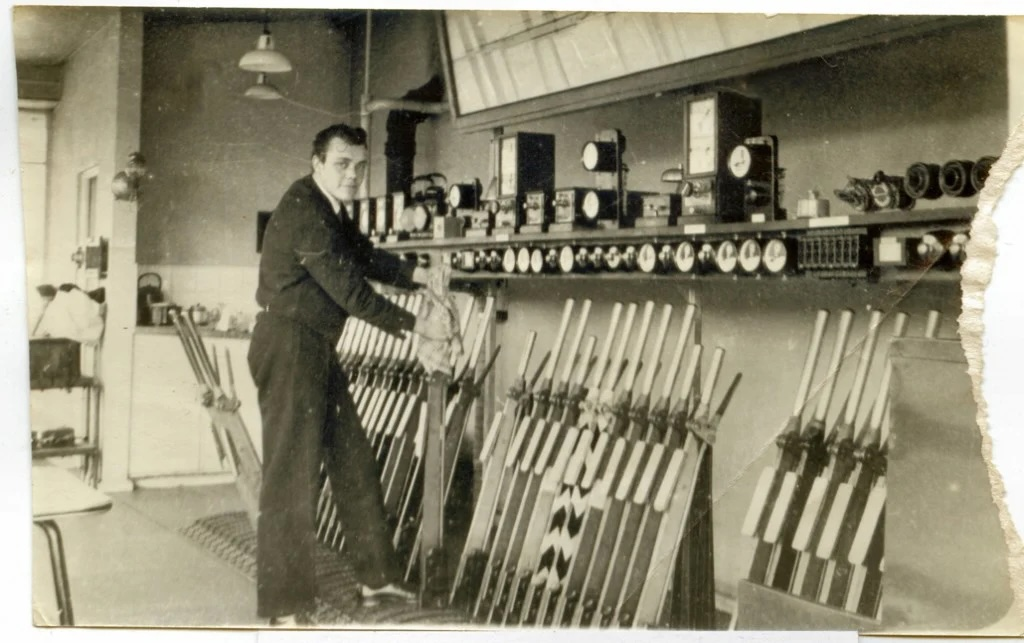
\includegraphics[width=10cm]{leversjpeg.jpg}
    \end{center}
\end{frame}

\begin{frame}{Partial Derivatives: Step 2}
    \begin{center}
        
\includegraphics[width=10cm]{guage.jpg}
    \end{center}
\end{frame}

\begin{frame}{Partial Derivatives}
    \textit{What happens to the gauge when you move one (1) lever?} \\

    \vspace{.5cm}
    This is contingent on two primary things:
    \begin{enumerate}
        \item What direction you move that lever
        \item Where all the other levers are set
    \end{enumerate}
\vspace{1cm}
    \textcolor{red}{These conditions are re-evaluated \textbf{\underline{at every point!}}}
\end{frame}

\begin{frame}{How Do We Approach This?}
    Multivariable calculus lends a very straightforward route for these solutions, both in differentiation and in integration:

    \emph{\textbf{Treat non-targeted variables as constants}}
\end{frame}

\begin{frame}{Working Through This}
    Consider a very simple example:

    \begin{align*}
        f(x,y) &= 2xy - x^2y^2
    \end{align*}

    Then, we can solve: \pause

    \begin{align*}
        \frac{\partial f(x,y)}{\partial x} &= 2y - 2xy^2 \\
        \frac{\partial f(x,y)}{\partial y} &= 2x - 2x^2y
    \end{align*}
\end{frame}

\begin{frame}{A Conceptual Question}
What must be true in a multi-dimensional local maxima (or minima)?
\end{frame}

\begin{frame}{Multivariate Optimization}
Total optimization in multivariable environments follows a simple -- even if technically exhausting -- algorithm:

\begin{enumerate}
    \item Find all critical points:
    \begin{enumerate}
        \item Solve $\frac{\partial f}{\partial x_i}$ for all $x_i$ and identify FOCs
        \item Solve FOCs as a system of equation to determine if any interior critical points exist
    \end{enumerate}
    \item Find endpoint maxima / minima:
    \begin{enumerate}
        \item Optimize edge values
    \end{enumerate}
    \item Compare values of all maxima / minima to determine extrema
\end{enumerate}
\end{frame}

\begin{frame}
    \begin{center}
        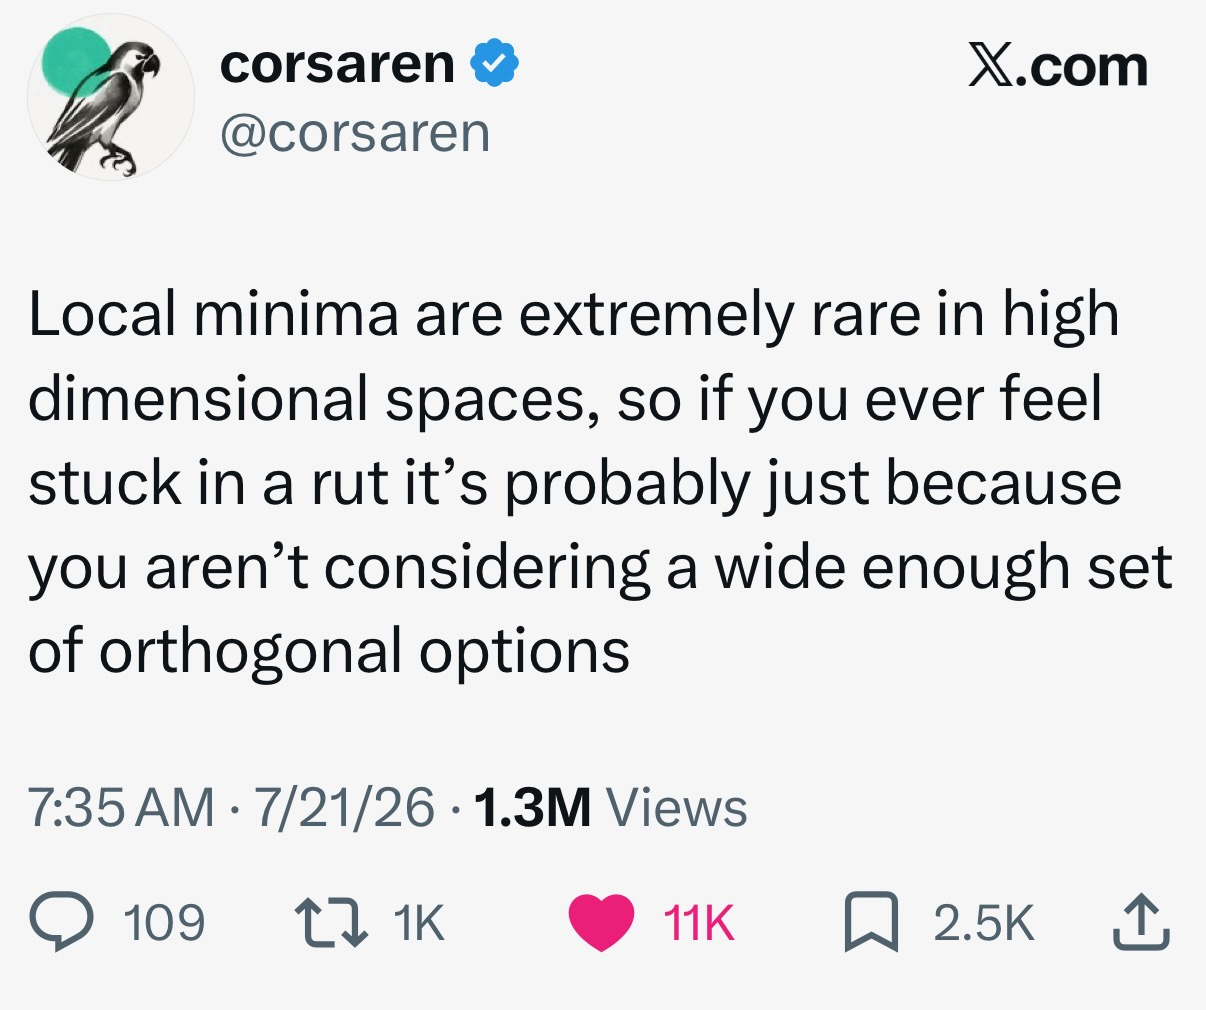
\includegraphics[width=10cm]{IMG_3850.jpeg}
    \end{center}
\end{frame}


\begin{frame}{A Very Common Optimization}
    From above: OLS = ``sum of least squares"... \\
    \vspace{1cm}
    That's just optimization! \\
    \vspace{1cm}
    Given $a < b < c$ and $f(a) < f(b) < f(c)$, \textbf{AND} with fixed $\hat{f}(0)=0$\footnote{you're welcome!}, how might we optimize our regression estimator (linear slope)?
\end{frame}

\begin{frame}{OLS Optimization}
    OLS solves the following:

    \[\min \sum \Big(\hat{f}(a) - f(a) \Big)^2 \quad \quad \implies \quad \quad \arg\min_m \sum \Big(f(m,a) - f(a)  \Big)^2\]

    We are holding $\hat{f}(0) = 0$, so $\hat{f}(x) = mx$. Then, we want to solve:

    \[\arg\min_m \sum_i \Big( m\cdot x_i - f(x) \Big)^2\]

    Expanded:

    \[\arg\min_m \Bigg[ \Big(ma - f(a) \Big)^2 + \Big(mb - f(b)\Big)^2 + \Big(mc - f(c)\Big)^2 \Bigg]\]
\end{frame}

\begin{frame}{OLS Optimization}
    \begin{align*}
        \frac{d}{dm}\Bigg[ \Big(ma - f(a) \Big)^2 + \Big(mb - f(b)\Big)^2 + \Big(mc - f(c)\Big)^2 \Bigg] \\= 2a\Big(ma-f(a)\Big) + 2b\Big(mb-f(b)\Big) + 2c\Big(mc-f(c)\Big)
    \end{align*}
    \[\frac{d}{dm} = 0 \implies 2a^2m + 2b^2 m + 2c^2m = 2af(a) + 2bf(b) + 2cf(c)\]
    \[2m(a^2 + b^2 + c^2) = 2\Big(af(a) + bf(b) + cf(c) \Big)\]
    \[m^* = \frac{af(a) + bf(b) + cf(c)}{a^2 + b^2 + c^2}\]
\end{frame}

%%MOVE TO MULTIVARIABLE OPTIMIZATION/CALCULUS%%

\begin{frame}{With One Little Difference}
    Now we know multivariable optimization. That's good! \\

    \vspace{1cm}

    Given $\bigg\{\Big(a,f(a)\Big), \Big(b, f(b)\Big), \Big(c,f(c)\Big) \bigg\}$ and \textbf{without} any assumption on $\hat{f}(0)$, let's derive an optimal OLS estimator (both coefficient and slope). \\

    \vspace{1cm}

    \textit{This only needs the sum rule and power rule!}
\end{frame}

\begin{frame}{The Math}
    Define $\hat{f}(x) \equiv mx + z$ for $m, z \in \mathbb{R}$. Then, our optimization problem becomes:

    \[\arg\min_{m,z} \Bigg[\Big(ma + z - f(a)\Big)^2  + \Big(mb + z - f(b)\Big)^2 + \Big(mc + z - f(c) \Big)^2\Bigg]\]
    \begin{align*}\frac{\partial}{\partial z} &= 2ma + 2mb + 2mc - 2f(a) - 2f(b) - 2f(c) + 6z \\ &=2m\Big(a + b + c\Big) - 2\Big( f(a) - f(b) - f(c) \Big) + 6z
    \end{align*}
    \[FOC: \frac{\partial}{\partial z} = 0 \implies z^* = \frac{-m(a+b+c) + f(a) + f(b) + f(c)}{3}\]
\end{frame}

\begin{frame}{The Math}
    \begin{align*}
    \frac{\partial}{\partial m} = 2m(a^2+b^2+c^2) + 2z(a+b+c) - 2\Big(af(a) + bf(b) + cf(c)\Big)
    \end{align*}
    \[FOC: \frac{\partial}{\partial m} = 0 \implies m^* = \frac{af(a) + bf(b) + cf(c) - z\Big(a+b+c\Big)}{a^2 + b^2 + c^2}\]
    \begin{align*}
        \Big(m^*, z^* \Big) = \Bigg(&\frac{af(a) + bf(b) + cf(c) - z\Big(a+b+c\Big)}{a^2 + b^2 + c^2}, \\ &\frac{-m(a+b+c) + f(a) + f(b) + f(c)}{3}\Bigg)
    \end{align*}
\end{frame}

\begin{frame}{The Math}
    We want to express this only in terms of $a,b,c$, so we substitute:
\begin{tiny}
    \begin{align*}
        &m^* = \frac{af(a) + bf(b) + cf(c) - \frac{-m^*(a+b+c) + f(a) + f(b) + f(c)}{3}\Big(a+b+c\Big)}{a^2 + b^2 + c^2} \\ \implies &m^* = \frac{3\Big(af(a) + bf(b) + cf(c) \Big) - \Big(a+b+c\Big)\Big(f(a) + f(b) + f(c)\Big)}{3\Big(a^2 + b^2 + c^2\Big) - \Big(a + b + c\Big)^2}
    \end{align*}
    \begin{align*}
        &z^* = \frac{-m^*\Big(a + b + c \Big) + f(a) + f(b) + f(c)}{3} \\
        \implies &z^* = \frac{-\bigg(\frac{3\Big(af(a) + bf(b) + cf(c) \Big) - \Big(a+b+c\Big)\Big(f(a) + f(b) + f(c)\Big)}{3\Big(a^2 + b^2 + c^2\Big) - \Big(a + b + c\Big)^2} \bigg) \Big(a + b + c \Big) + f(a) + f(b) + f(c)}{3}
    \end{align*}
    We could simplify further, but have no need
\end{tiny}
\end{frame}

\begin{frame}{Run A Test}
    Set the following three data points: $(1,2), (2,3),(3,5)$. Then, evaluate:

    \[(m^*, z^*) = \]
\end{frame}



\end{document}